\chapter{Conos de luz, geodésicas y el horizonte de Schwarzschild}

El problema del horizonte comienza con una distinción ya presente en la relatividad especial. Dos sucesos próximos pueden estar separados en una dirección temporal, espacial o lumínica. La curvatura no elimina esta clasificación. Hace que el cono de luz sea un objeto local, distinto en cada suceso, y que la propia métrica sea dinámica. Una vez conocida la métrica, el movimiento de una partícula en caída libre se obtiene del mismo principio del tiempo propio que describe una partícula relativista libre en el espacio-tiempo plano.

Usaremos ese principio dos veces. Primero, debe reproducir el movimiento newtoniano en un campo débil. Después, se aplicará a la métrica de Schwarzschild, donde el significado del tiempo, la distancia radial y la velocidad se vuelve inesperadamente sutil.

\section{Intervalos temporales, espaciales y lumínicos}

En el espacio-tiempo plano, con \(c=1\), el elemento de tiempo propio es
\begin{equation}
d\tau^2=dt^2-dx^2-dy^2-dz^2.
\label{eq:l5-minkowski-proper-time}
\end{equation}
Conviene restituir \(c\) cuando se considera una aproximación no relativista:
\begin{equation}
d\tau^2
=dt^2-\frac{dx^2+dy^2+dz^2}{c^2}.
\label{eq:l5-minkowski-c}
\end{equation}
La notación \(d\tau^2\) no garantiza que el lado derecho sea positivo. Su signo clasifica el desplazamiento:
\begin{align}
d\tau^2>0
&\quad\Longleftrightarrow\quad \text{time-like},\\
d\tau^2=0
&\quad\Longleftrightarrow\quad \text{light-like},\\
d\tau^2<0
&\quad\Longleftrightarrow\quad \text{space-like}.
\end{align}
Para un desplazamiento espacial, es conveniente definir la distancia propia positiva
\begin{equation}
ds^2=-d\tau^2
=dx^2+dy^2+dz^2-dt^2
\qquad(c=1).
\label{eq:l5-proper-distance}
\end{equation}

El cono de luz organiza estas tres posibilidades. Su superficie, y no su interior, está formada por las direcciones lumínicas. Las direcciones temporales quedan dentro del cono y las espaciales, fuera. Las mitades superior e inferior representan los conos de luz futuro y pasado.

\begin{figure}[htbp]
\centering
\includegraphics[width=0.82\textwidth]{lecture_05_figure_02.png}
\caption{Tiempo propio, distancia propia y cono causal representados juntos en la pizarra. Los rayos de luz ocupan el cono mismo; el interior es temporal y el exterior, espacial.}
\lectureframe{00:05:44}
\end{figure}

\begin{figure}[htbp]
\centering
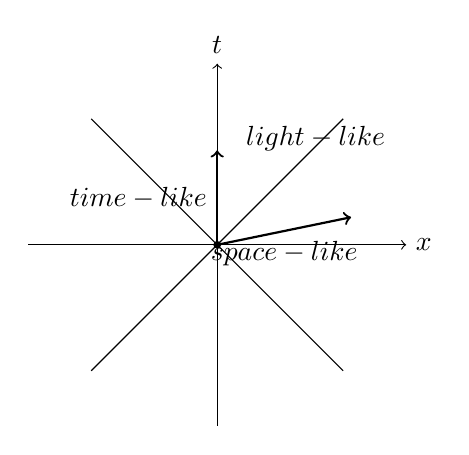
\begin{tikzpicture}[scale=1.0]
\draw[->] (0,-2.3) -- (0,2.3) node[above] {\(t\)};
\draw[->] (-2.4,0) -- (2.4,0) node[right] {\(x\)};
\draw (-1.6,1.6) -- (0,0) -- (1.6,1.6);
\draw (-1.6,-1.6) -- (0,0) -- (1.6,-1.6);
\fill (0,0) circle (1.4pt);
\draw[->,thick] (0,0) -- (0,1.2)
  node[midway,left] {\(\text{time-like}\)};
\draw[->,thick] (0,0) -- (1.7,0.35)
  node[midway,below] {\(\text{space-like}\)};
\node at (1.25,1.35) {\(\text{light-like}\)};
\end{tikzpicture}
\caption{La clasificación causal en una sección bidimensional del espacio-tiempo.}
\end{figure}

Estos intervalos tienen una definición operacional. El tiempo propio es lo que marca un reloj llevado a lo largo de una línea de universo temporal. La distancia propia es lo que mide un conjunto apropiado de varas métricas entre sucesos separados espacialmente. No son meros nombres para los signos de una forma cuadrática.

\section{Firma lorentziana y un cono en cada suceso}

Con la convención tensorial de signos mayormente positivos, la métrica plana tiene componentes
\begin{equation}
\eta_{\mu\nu}=\operatorname{diag}(-1,1,1,1),
\label{eq:l5-eta}
\end{equation}
y
\begin{equation}
d\tau^2=-\eta_{\mu\nu}\,dx^\mu dx^\nu.
\label{eq:l5-proper-time-eta}
\end{equation}
La matriz mostrada expresa un tensor de rango dos en una base especialmente sencilla. Su característica invariante es su firma: una dirección negativa y tres positivas,
\begin{equation}
\operatorname{signature}(\eta)=(-,+,+,+).
\label{eq:l5-lorentz-signature}
\end{equation}
Una métrica con dos signos negativos tendría dos direcciones temporales. Estas firmas pueden estudiarse matemáticamente, pero no describen el espacio-tiempo que suponemos aquí.

En un espacio-tiempo curvo, los componentes varían:
\begin{equation}
g_{\mu\nu}=g_{\mu\nu}(x).
\label{eq:l5-position-metric}
\end{equation}
La métrica debe seguir teniendo firma lorentziana en cada suceso. Por consiguiente, cada suceso tiene sus propias direcciones temporales, su frontera lumínica y sus direcciones espaciales. Un dibujo en coordenadas puede mostrar conos inclinados o deformados de un punto a otro, pero la clasificación causal se mantiene.

\begin{figure}[htbp]
\centering
\includegraphics[width=0.86\textwidth]{lecture_05_figure_03.png}
\caption{La métrica dependiente de la posición \(g_{\mu\nu}(x)\), las etiquetas causales y los esquemas de conos de luz locales.}
\lectureframe{00:09:41}
\end{figure}

\begin{figure}[htbp]
\centering
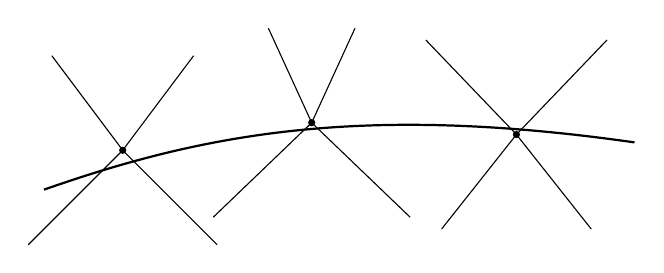
\begin{tikzpicture}[scale=1.0]
\draw[thick] (-4,-0.5) .. controls (-2,0.2) and (0,0.6) .. (3.5,0.1);
\foreach \x/\y/\a/\b in {-3/0/0.9/1.2, -0.6/0.35/0.55/1.25,
                          2.0/0.2/1.15/0.95} {
  \fill (\x,\y) circle (1.3pt);
  \draw (\x,\y) -- ++(-\a,1.2);
  \draw (\x,\y) -- ++(\a,1.2);
  \draw (\x,\y) -- ++(-\b,-1.2);
  \draw (\x,\y) -- ++(\b,-1.2);
}
\end{tikzpicture}
\caption{Conos locales vecinos. Su forma en coordenadas puede cambiar sin alterar qué vectores son temporales, lumínicos o espaciales.}
\end{figure}

\begin{classroomqa}
\audiencequestion{¿El único autovalor negativo selecciona una dirección temporal única?}
\lecturerresponse{Una base que diagonaliza la matriz mostrada tiene una dirección de base negativa, pero eso no selecciona un observador preferido ni una única flecha física. Las transformaciones de Lorentz mezclan la coordenada temporal con las coordenadas espaciales, y todo vector dentro del cono es temporal. El objeto invariante es el cono junto con la firma de un signo negativo y tres positivos, no un vector temporal distinguido.
\lecturetimestamp{00:12:17--00:17:24}}
\end{classroomqa}

\begin{classroomqa}
\audiencequestion{¿Por qué pueden tener formas distintas dos dibujos del cono local?}
\lecturerresponse{Las coordenadas pueden cambiar el dibujo. Por ejemplo, sustituir \(x\) por una coordenada reescalada cambia la pendiente numérica asignada a un rayo de luz y, por tanto, hace que el cono parezca más estrecho o más ancho. Otras coordenadas más generales pueden inclinarlo. Se representan el mismo suceso y las mismas relaciones causales. En un espacio-tiempo curvo, además, los conos de sucesos distintos pertenecen a espacios tangentes distintos, por lo que compararlos requiere la métrica y una regla de transporte.
\lecturetimestamp{00:13:37--00:15:59}}
\end{classroomqa}

\section{Geodésicas como problema variacional}

Una partícula en movimiento libre sigue una geodésica del espacio-tiempo. En forma diferencial, usando un parámetro afín \(\lambda\),
\begin{equation}
\frac{d^2x^\mu}{d\lambda^2}
+\Gamma^\mu{}_{\rho\sigma}
\frac{dx^\rho}{d\lambda}
\frac{dx^\sigma}{d\lambda}=0.
\label{eq:l5-geodesic}
\end{equation}
La conexión indica cómo debe mantenerse paralelo a sí mismo el vector tangente mientras se mueve la partícula.

Hay otra formulación que suele facilitar los cálculos. En un espacio riemanniano con métrica \(g_{mn}\), la longitud de una curva es
\begin{equation}
s=\int ds
=\int\sqrt{g_{mn}\,dx^m dx^n}.
\label{eq:l5-spatial-length}
\end{equation}
La geodésica hace estacionaria esta longitud frente a pequeñas variaciones de la trayectoria con los extremos fijos. La integral es simplemente la suma de longitudes infinitesimales a lo largo de la curva, y su ecuación de Euler--Lagrange es una ecuación diferencial de segundo orden, análoga en su forma a una ley de fuerzas.

Para una línea de universo temporal, la longitud espacial se sustituye por el tiempo propio:
\begin{equation}
\tau
=\int\sqrt{-g_{\mu\nu}\,dx^\mu dx^\nu}.
\label{eq:l5-proper-time-functional}
\end{equation}
Una geodésica temporal hace estacionario \(\tau\) y, para trayectorias cercanas en caída libre y antes de que aparezcan puntos conjugados, lo maximiza localmente. Al multiplicarlo por \(-m\) se obtiene la acción de la partícula
\begin{equation}
A=-m\tau
=-m\int\sqrt{-g_{\mu\nu}\,dx^\mu dx^\nu}.
\label{eq:l5-particle-action}
\end{equation}
Así, la misma trayectoria minimiza localmente \(A=-m\tau\). La distinción entre un tiempo propio estacionario y el signo de la acción elegida resuelve la aparente ambigüedad entre mínimo y máximo.

\section{Del tiempo propio a un lagrangiano ordinario}

La acción de \eqref{eq:l5-particle-action} es geométrica, pero puede expresarse en la forma familiar de la mecánica. Parametrizamos la línea de universo con la coordenada \(t\), dividimos cada diferencial por \(dt\) y sacamos de la raíz el factor restante \(dt\):
\begin{align}
A
&=-m\int\sqrt{-g_{\mu\nu}(x)\,dx^\mu dx^\nu}\\
&=-m\int
\sqrt{-g_{\mu\nu}(x)
\frac{dx^\mu}{dt}\frac{dx^\nu}{dt}}\,dt.
\label{eq:l5-action-t}
\end{align}
Para la componente temporal, \(dt/dt=1\); las componentes espaciales son velocidades coordenadas ordinarias. Por tanto, podemos escribir
\begin{equation}
\begin{aligned}
A&=\int L\,dt,\\
L&=-m\sqrt{-g_{\mu\nu}(x)\dot x^\mu\dot x^\nu},\\
\dot x^\mu&=\frac{dx^\mu}{dt}.
\end{aligned}
\label{eq:l5-relativistic-lagrangian}
\end{equation}

\begin{figure}[htbp]
\centering
\includegraphics[width=0.88\textwidth]{lecture_05_figure_05.png}
\caption{Conversión de la acción de la línea de universo a la forma convencional \(A=\int L\,dt\).}
\lectureframe{00:27:00}
\end{figure}

\begin{figure}[htbp]
\centering
\includegraphics[width=0.88\textwidth]{lecture_05_figure_06.png}
\caption{Estado posterior de la pizarra, con el lagrangiano relativista despejado.}
\lectureframe{00:28:59}
\end{figure}

\begin{classroomqa}
\audiencequestion{¿Deberían ser griegos los índices del espacio-tiempo en esta acción?}
\lecturerresponse{Sí. Los índices griegos recorren el tiempo y todas las coordenadas espaciales. Los índices latinos pueden reservarse para las coordenadas espaciales cuando resulte útil distinguirlas.
\lecturetimestamp{00:25:53--00:26:03}}
\end{classroomqa}

\begin{classroomqa}
\audiencequestion{¿Por qué se llama lagrangiano a la expresión con raíz cuadrada?}
\lecturerresponse{Una vez escrita la acción como \(A=\int L\,dt\), el integrando es el lagrangiano. No se trata solo de una definición: al variar ese integrando se obtienen las ecuaciones de Euler--Lagrange
\[
\frac{d}{dt}
\left(\frac{\partial L}{\partial\dot x^\mu}\right)
=\frac{\partial L}{\partial x^\mu},
\]
que son equivalentes a la ecuación geodésica si se trata el parámetro de manera coherente.
\lecturetimestamp{00:28:36--00:29:02}}
\end{classroomqa}

Para una partícula masiva, la línea de universo es temporal, de modo que la cantidad bajo la raíz cuadrada es positiva. Una trayectoria espacial describiría un movimiento superlumínico, no la trayectoria de una partícula masiva ordinaria. Dada una métrica, ahora se puede obtener la trayectoria de la partícula calculando los símbolos de Christoffel y usando \eqref{eq:l5-geodesic}, o aplicando Euler--Lagrange a \eqref{eq:l5-relativistic-lagrangian}. Demostrar que ambos métodos son equivalentes es un ejercicio útil; el método de la acción suele ser más breve.

\section{El límite newtoniano}

Consideremos el campo gravitatorio débil y estático fuera de una fuente esférica. Partamos del espacio-tiempo plano y permitamos que el coeficiente de \(dt^2\) difiera ligeramente de la unidad:
\begin{equation}
d\tau^2
=\left(1+\frac{2u(\mathbf{x})}{c^2}\right)dt^2
-\frac{d\mathbf{x}^2}{c^2},
\label{eq:l5-weak-metric}
\end{equation}
donde \(u\) debe convertirse en el potencial newtoniano. Este planteamiento debe comprobarse, no limitarse a bautizarlo.

La acción de la partícula, con dimensiones físicas, es
\begin{equation}
A=-mc^2\int
\sqrt{1+\frac{2u}{c^2}
-\frac{\dot{\mathbf{x}}^{\,2}}{c^2}}\,dt.
\label{eq:l5-weak-action}
\end{equation}
Tanto \(u/c^2\) como \(\dot{\mathbf{x}}^{\,2}/c^2\) son pequeños. Conservando sus contribuciones de primer orden,
\begin{equation}
\sqrt{1+\epsilon}
=1+\frac{\epsilon}{2}+O(\epsilon^2),
\qquad
\epsilon=\frac{2u-\dot{\mathbf{x}}^{\,2}}{c^2},
\end{equation}
se obtiene
\begin{align}
L
&=-mc^2
\sqrt{1+\frac{2u-\dot{\mathbf{x}}^{\,2}}{c^2}}\\
&=-mc^2-mu+\frac{m}{2}\dot{\mathbf{x}}^{\,2}\\
&\quad+O\!\left(c^{-2}
 [u^2+u\dot{\mathbf{x}}^{\,2}+\dot{\mathbf{x}}^{\,4}]\right).
\label{eq:l5-newton-expansion}
\end{align}
El término constante de energía en reposo no afecta las ecuaciones de movimiento. Lo que queda es
\begin{equation}
L_{\mathrm{nr}}
=\frac{m}{2}\dot{\mathbf{x}}^{\,2}-m u(\mathbf{x}),
\label{eq:l5-newton-lagrangian}
\end{equation}
y, por tanto,
\begin{equation}
m\ddot{\mathbf{x}}=-m\boldsymbol{\nabla}u.
\label{eq:l5-newton-equation}
\end{equation}
La masa de prueba se cancela, como debe ocurrir en la caída libre universal. La energía potencial es \(m u\), mientras que la aceleración es independiente de \(m\).

Así, hemos identificado la relación principal en el campo débil
\begin{equation}
g_{00}=1+\frac{2u}{c^2}+O(c^{-4}).
\label{eq:l5-g00-newton}
\end{equation}
Fuera de una masa esférica \(M\),
\begin{equation}
u(r)=-\frac{GM}{r},
\qquad
g_{00}=1-\frac{2GM}{rc^2}+O(c^{-4}).
\label{eq:l5-g00-spherical}
\end{equation}
Esto determina la primera corrección a la componente temporal. Aún no determina la métrica completa en el campo fuerte.

\section{Coordenadas esféricas y la primera conjetura de Schwarzschild}

Las coordenadas esféricas son naturales para una fuente central. En la clase se mide \(\theta\) desde el plano ecuatorial y no desde el polo, por lo que el elemento de línea angular es
\begin{equation}
d\Omega^2=d\theta^2+\cos^2\theta\,d\phi^2.
\label{eq:l5-angular-metric}
\end{equation}
Con esta convención,
\begin{equation}
d\mathbf{x}^2=dr^2+r^2d\Omega^2.
\label{eq:l5-flat-spherical}
\end{equation}
La elección de esta coordenada \(\theta\), análoga a una latitud, no tiene consecuencias físicas; con el ángulo polar más habitual, \(\cos^2\theta\) se sustituiría por \(\sin^2\theta\).

Al insertar el coeficiente temporal newtoniano y dejar plana la métrica espacial, se obtiene la primera conjetura
\begin{equation}
\begin{aligned}
d\tau^2
&=\left(1-\frac{r_s}{r}\right)dt^2
-\frac{1}{c^2}\left(dr^2+r^2d\Omega^2\right),\\
r_s&=\frac{2GM}{c^2}.
\end{aligned}
\label{eq:l5-naive-schwarzschild}
\end{equation}
Esta no puede ser la respuesta exacta. Para \(r<r_s\), el coeficiente de \(dt^2\) cambia de signo mientras todos los coeficientes espaciales siguen siendo negativos en la convención del tiempo propio. La métrica perdería la firma de una dirección temporal y tres espaciales.

Las ecuaciones de campo en el vacío proporcionan el coeficiente radial requerido:
\begin{equation}
\boxed{
d\tau^2
=\left(1-\frac{r_s}{r}\right)dt^2
-\frac{dr^2}{c^2\left(1-r_s/r\right)}
-\frac{r^2}{c^2}d\Omega^2.
}
\label{eq:l5-schwarzschild}
\end{equation}
Esta es la métrica exterior de Schwarzschild. Cuando \(r\) atraviesa \(r_s\), los coeficientes \(t\) y \(r\) cambian de signo a la vez, y se conserva la firma lorentziana. En las coordenadas de Schwarzschild, la coordenada radial se vuelve temporal en el interior y la coordenada \(t\) se vuelve espacial. Este intercambio señala un fallo de la carta de coordenadas en el horizonte, no un fallo local de la geometría del espacio-tiempo.

\begin{classroomqa}
\audiencequestion{¿Cuánto tarda un objeto en caída en atravesar el horizonte?}
\lecturerresponse{Según el tiempo coordenado de Schwarzschild \(t\) que usa un observador distante, el cruce se prolonga hasta un tiempo infinito. Según el tiempo propio que marca el reloj del objeto en caída, ocurre en un tiempo finito. La distinción entre estos relojes es el problema central del horizonte.
\lecturetimestamp{00:54:45--00:55:35}}
\end{classroomqa}

\begin{classroomqa}
\audiencequestion{¿Por qué modificar el coeficiente radial y no otra parte de la métrica?}
\lecturerresponse{La métrica debe conservar la firma lorentziana, la simetría esférica distingue la dirección radial de la esfera angular, y las ecuaciones de campo en el vacío determinan con precisión el factor recíproco. La firma indica dónde buscar; las ecuaciones de Einstein dan el resultado exacto.
\lecturetimestamp{00:55:35--00:56:01}}
\end{classroomqa}

Para la Tierra, \(r_s\) es apenas del orden de un centímetro, muy por debajo de la superficie del cuerpo material. La métrica exterior en el vacío no es válida allí, así que la Tierra no tiene horizonte de Schwarzschild. En el interior debe sustituirse por una solución interior, que ha de empalmarse con la exterior en la superficie.

\begin{classroomqa}
\audiencequestion{Si \(t\) y \(r\) intercambian sus papeles como coordenadas, ¿qué ocurre con un reloj ordinario?}
\lecturerresponse{El reloj sigue midiendo el tiempo propio a lo largo de una línea de universo temporal. No sabe que una coordenada elegida se ha vuelto incómoda. Un sistema regular de coordenadas en caída libre muestra una geometría local suave y una propagación local ordinaria de la luz a través del horizonte.
\lecturetimestamp{00:56:35--00:57:50}}
\end{classroomqa}

\subsection{Por qué la corrección radial no apareció en la ecuación de Newton}

La métrica exacta modifica el coeficiente radial ya en primer orden en el potencial:
\begin{equation}
\frac{1}{1-r_s/r}
=1+\frac{r_s}{r}
+O\!\left(\frac{r_s^2}{r^2}\right)
=1-\frac{2u}{c^2}+O(c^{-4}).
\label{eq:l5-radial-expansion}
\end{equation}
¿Por qué fue legítimo ignorar ese cambio en la derivación newtoniana? En la acción de la partícula multiplica a \(\dot r^2/c^2\). Por tanto, su primera corrección es proporcional a
\begin{equation}
\frac{u\,\dot r^2}{c^4},
\end{equation}
que es de orden superior al retenido en \eqref{eq:l5-newton-expansion}. La corrección radial es despreciable en la prueba newtoniana de movimiento lento, pero se vuelve decisiva para el movimiento relativista y cerca del horizonte. Esto es una advertencia útil: un término demasiado pequeño para una aproximación puede controlar el fenómeno de interés en otra.

\section{Caída radial en el tiempo de Schwarzschild}

Fijemos \(c=1\) y estudiemos primero el movimiento radial. Las órbitas circulares también son importantes, pero requieren los términos angulares y las dejamos para más adelante. El movimiento radial se parece menos a una órbita que a una caída directa hacia la fuente, y permite estudiar el comportamiento del horizonte con el menor álgebra posible.

\begin{classroomqa}
\audiencequestion{¿De quién es el tiempo que aparece en la velocidad radial?}
\lecturerresponse{El punto sobre la variable indica derivación respecto al tiempo coordenado de Schwarzschild \(t\), normalizado al observador estático distante. El reloj de pulsera del observador en caída mide el tiempo propio \(\tau\). Confundir ambos convertiría una afirmación sobre coordenadas en una afirmación local falsa.
\lecturetimestamp{01:04:03--01:04:47}}
\end{classroomqa}

Para \(d\Omega=0\), definamos
\begin{equation}
a(r)=1-\frac{r_s}{r}.
\label{eq:l5-a-def}
\end{equation}
La métrica radial y el lagrangiano son
\begin{align}
d\tau^2&=a\,dt^2-\frac{dr^2}{a},\\
L&=-m\sqrt{a-\frac{\dot r^2}{a}},
\qquad
\dot r=\frac{dr}{dt}.
\label{eq:l5-radial-lagrangian}
\end{align}
Como \(L\) no depende explícitamente de \(t\), su hamiltoniano se conserva. El momento radial es
\begin{equation}
p_r=\frac{\partial L}{\partial\dot r}
=\frac{m\dot r}{a\sqrt{a-\dot r^2/a}},
\label{eq:l5-radial-momentum}
\end{equation}
y
\begin{align}
H
&=p_r\dot r-L\\
&=\frac{ma}{\sqrt{a-\dot r^2/a}}
=E.
\label{eq:l5-radial-energy}
\end{align}
Al despejar la velocidad coordenada se obtiene
\begin{equation}
\boxed{
\dot r^2
=a^2\left(1-\frac{m^2}{E^2}a\right).
}
\label{eq:l5-radial-velocity}
\end{equation}
El cálculo en la pizarra examina varias expresiones algebraicas intermedias; la expresión recuadrada es el resultado coherente.

Cuando \(r\) se aproxima a \(r_s\), \(a(r)\) se aproxima a cero, mientras que el factor entre paréntesis se aproxima a uno. Por tanto,
\begin{equation}
\frac{dr}{dt}
\sim -\left(1-\frac{r_s}{r}\right)
\longrightarrow 0
\qquad(r\longrightarrow r_s^+)
\label{eq:l5-infall-freeze}
\end{equation}
para una partícula que cae hacia dentro. En el tiempo de Schwarzschild, la partícula parece ralentizarse y quedar congelada justo fuera del horizonte.

\begin{classroomqa}
\audiencequestion{¿Significa el valor decreciente de \(dr/dt\) que la gravedad se ha vuelto repulsiva?}
\lecturerresponse{No. La partícula no recibe localmente un empuje hacia fuera. La coordenada \(t\) resulta cada vez menos adecuada para describir el cruce, por lo que el avance radial por unidad de \(t\) tiende a cero. La aceleración propia a lo largo de la línea de universo en caída libre sigue siendo nula, y el horizonte se alcanza en un tiempo propio finito.
\lecturetimestamp{01:14:18--01:16:38}}
\end{classroomqa}

En efecto, cerca del horizonte,
\begin{equation}
\frac{dt}{dr}
\sim-\frac{1}{1-r_s/r}
=-\frac{r}{r-r_s}.
\end{equation}
Su integral diverge logarítmicamente. Esto demuestra que el tiempo de Schwarzschild es infinito sin implicar que el reloj del objeto en caída registre un tiempo infinito.

\section{Rayos de luz radiales}

La luz permite hacer el mismo cálculo de la forma más breve. Para un rayo nulo radial,
\begin{equation}
d\tau^2
=a\,dt^2-\frac{dr^2}{a}=0.
\end{equation}
Por tanto,
\begin{equation}
\boxed{
\frac{dr}{dt}
=\pm a(r)
=\pm\left(1-\frac{r_s}{r}\right).
}
\label{eq:l5-radial-light}
\end{equation}
El signo positivo describe un rayo saliente y el negativo, uno entrante. Ambas velocidades coordenadas tienden a cero en el horizonte.

\begin{classroomqa}
\audiencequestion{¿Qué velocidad da la fórmula lejos de la fuente?}
\lecturerresponse{Cuando \(r\) tiende a infinito, \(a(r)\) tiende a uno, de modo que \(dr/dt\) tiende a \(\pm1\), o a \(\pm c\) al restituir las unidades.
\lecturetimestamp{01:21:01--01:21:29}}
\end{classroomqa}

La relatividad general suele ser así: sus principios caben en unas pocas líneas, mientras que las coordenadas y los cálculos se complican. La ecuación \eqref{eq:l5-radial-light} es sencilla, pero interpretar su anulación cerca de \(r_s\) exige cuidado. Se trata de una velocidad coordenada, no de la velocidad que mide un observador inercial local.

\section{Lo que observa un observador distante}

\begin{classroomqa}
\audiencequestion{¿Puede escapar la luz emitida cerca del horizonte y se trata de radiación de Hawking?}
\lecturerresponse{Un rayo clásico saliente, emitido justo fuera del horizonte, puede avanzar hacia fuera, pero su velocidad coordenada de Schwarzschild es inicialmente extremadamente pequeña y la señal llega al infinito solo tras un retraso y un corrimiento al rojo muy pronunciados. Un rayo situado en el horizonte permanece en él en estas coordenadas; un rayo en el interior no puede escapar. La radiación de Hawking es un efecto de teoría cuántica de campos asociado a la geometría exterior, no un rayo de luz clásico que ascienda desde el interior, y no se deriva del cálculo presente.
\lecturetimestamp{01:22:08--01:24:28}}
\end{classroomqa}

\begin{classroomqa}
\audiencequestion{Si un fotón parece casi inmóvil, ¿empieza a parecer masivo?}
\lecturerresponse{No. Un observador local en caída libre siempre mide que el fotón se mueve a \(c\). Solo la razón entre coordenadas \(dr/dt\) tiende a cero. La masa, el carácter nulo y la velocidad local de la luz no cambian por una carta de coordenadas inadecuada.
\lecturetimestamp{01:24:31--01:25:26}}
\end{classroomqa}

La expresión de Schwarzschild usada aquí es una solución exterior en el vacío. Una estrella, un planeta o una nube en colapso tienen una métrica interior distinta, que debe empalmarse con la exterior. Si la superficie material permanece fuera de \(r_s\), como ocurre con la Tierra por un margen enorme, el horizonte de coordenadas exterior queda fuera del dominio en que puede prolongarse la fórmula del vacío a través de la materia. Si el cuerpo colapsa hasta quedar dentro de su radio de Schwarzschild, el horizonte pasa a formar parte del espacio-tiempo físico.

\begin{classroomqa}
\audiencequestion{Si un observador exterior nunca ve cruzar a la materia, ¿cómo puede formarse o crecer un agujero negro?}
\lecturerresponse{La premisa trata el tiempo de Schwarzschild como si fuera un reloj físico global en el horizonte. La conclusión de que, por tanto, un agujero negro nunca puede crecer parece plausible, pero es errónea. Una respuesta completa requiere coordenadas regulares que atraviesen el horizonte y la geometría causal global del colapso; esa explicación se pospone a la siguiente etapa del curso.
\lecturetimestamp{01:27:57--01:29:36}}
\end{classroomqa}

\begin{classroomqa}
\audiencequestion{¿Qué indicaría un radar de velocidad para un automóvil que cae hacia el horizonte?}
\lecturerresponse{La velocidad coordenada primero aumenta mientras cae el automóvil; después alcanza un máximo y disminuye hacia cero. Los pulsos de radar enviados más tarde todavía pueden alcanzar el automóvil fuera del horizonte, pero el tiempo de ida y vuelta aumenta progresivamente. La señal de retorno sufre un corrimiento al rojo cada vez mayor, y la imagen parece ralentizarse y comprimirse cerca de \(r_s\). Esta no es una imagen local fiable de lo que experimenta el conductor; este atraviesa el horizonte en un tiempo propio finito.
\lecturetimestamp{01:29:39--01:32:14}}
\end{classroomqa}

\begin{classroomqa}
\audiencequestion{¿La velocidad de la luz es constante solo en la relatividad especial?}
\lecturerresponse{También es constante en todo sistema de referencia inercial local de la relatividad general. Un observador en caída, con relojes locales y varas métricas, mide que un fotón cercano se mueve a \(c\). Las velocidades coordenadas, como \(dr/dt\), pueden variar porque \(r\) y \(t\) no son las lecturas de un único laboratorio inercial local en todo el espacio-tiempo.
\lecturetimestamp{01:32:20--01:34:20}}
\end{classroomqa}

\section{Preguntas que van más allá del cálculo de Schwarzschild}

\begin{classroomqa}
\audiencequestion{¿Qué podría significar unificar la gravedad con las demás fuerzas?}
\lecturerresponse{Una posibilidad geométrica consiste en ampliar el espacio-tiempo con direcciones compactas adicionales. Entonces, los componentes de una métrica de dimensión superior pueden aparecer en cuatro dimensiones como campos gauge y campos escalares, mientras que el momento en una dirección extra puede aparecer como una carga. Esta es una pista estructural asociada a las ideas de Kaluza--Klein, no una unificación completa en esta clase.
\lecturetimestamp{01:34:22--01:36:08}}
\end{classroomqa}

\begin{classroomqa}
\audiencequestion{¿Podrían tener distintas regiones o universos firmas métricas diferentes?}
\lecturerresponse{La relatividad general clásica suele fijar una firma lorentziana no degenerada. Cambiarla exigiría que la métrica pasara por una configuración degenerada, donde falla la descripción clásica estándar. La gravedad cuántica podría exigir un lenguaje más amplio, pero no existe aquí una teoría establecida que prediga regiones físicas con cambio de firma.
\lecturetimestamp{01:36:08--01:38:08}}
\end{classroomqa}

\begin{classroomqa}
\audiencequestion{¿Cómo encontró Schwarzschild esta solución mientras prestaba servicio durante la Primera Guerra Mundial?}
\lecturerresponse{La idea que se plantea en clase es tanto humana como histórica: Schwarzschild era astrónomo y matemático de gran talento, y trabajar con las nuevas ecuaciones de Einstein le ofrecía un refugio intelectual en medio del servicio durante la guerra.
\lecturetimestamp{01:38:11--01:39:02}}
\end{classroomqa}

La lección central queda ahora lo bastante clara como para seguir adelante. La métrica determina tanto los conos causales como el movimiento libre. Su componente temporal en el campo débil contiene el potencial de Newton, mientras que su forma exacta de Schwarzschild da un horizonte de coordenadas en \(r=r_s\). El tiempo de Schwarzschild prolonga el cruce hasta el infinito; el tiempo propio del observador en caída, no. El siguiente problema consiste en resolver globalmente este contraste y explicar cómo se forma un agujero negro pese a que la imagen distante parece congelada.